\section{Motivation}
In our universe, we observe a surplus of particles over antiparticles that is called \textit{baryon asymmetry}. A key aspect of this matter-antimatter 
problem is the violation of \textit{CP} symmetry that occures in weak interactions. In this experiment, the decays of $B$ mesons measured by the LHCb experiment
are analyzed to calculate the \textit{CP} asymmetry.

\section{Theory}
\label{sec:Theory}
In 1964, \textit{CP} violation was observed for the first time by Cronin and Fitch~\cite{Cronin_Fitch_cpv} in the decay of neutral Kaons. At this time, the Standard Model of 
particle physics did not provide methods to describe \textit{CP} violation. This chapter focuses on establishing a connection between the baryon asymmetry
and the violation of the \textit{CP} symmetry. Moreover, the theory behind \textit{CP} violation is explained.

\subsection{Sakharov conditions}
\label{sec:sakharov_conditions}
For a higher production rate of matter over antimatter, three conditions must be fullfilled. These conditions are referred to as the \textit{Sakharov conditions},
named after the physicist Andrei Sakharov who proposed these criteria in 1966~\cite{Sakharov_conditions}.
First, a violation of the baryon number $B$ is needed. This is in disagreement with the Standard Model as we know it today but extensions of it could
allow for baryon number violation. \\
Second, both the charge symmetry $C$ and the combination of the charge and parity symmetries \textit{CP} need to be violated. The \textit{CP} violation is the topic
of this lab course and is explained in detail in the following sections. \\
The third conditon states that the violation of the baryon number (first conditon) needs to occur out of thermal equilibrium. If this was not the true, any 
baryon number asymmetry would lead to a corresponding reverse process and thus no overall asymmetry could be observed. Consequently, the universe is not in
a state of thermal equilibrium.

\subsection{\textit{CP} violation in the weak interaction}
\label{sec:cpv}
Before 1970, the weak interaction theory was based on Nicola Cabibbo's notation of the unitary symmetry~\cite{Cabibbo_paper} leading to quark mixing via 
the Cabibbo angle. This notation described how the weak interaction causes transitions between different quark flavors via  
\begin{align*}
    u \leftrightarrow d\cdot\cos(\theta_{\mathrm{C}}) \quad \text{and} \quad u \leftrightarrow s\cdot\sin(\theta_{\mathrm{C}}).
\end{align*}
At this time, only three quarks (u,d,s) were known to be part of the Standard Model.
This theory faced issues with renormalizability, failing to adequately describe certain decays or particle interactions. 
In 1970, Glashow, Iliopoulos, and Maiani proposed a new weak interaction theory~\cite{GIM_paper}, introducing a fourth quark (charm) and one vector boson~($Z_0$). 
This model helped address these problems and allowed for the integration of the previously predicted boson and the unification with the electroweak interaction.
A few years later, in 1973, Kobayashi and Maskawa further refined the theory of the weak interaction by postullating a third generation of quarks~\cite{KM_paper}.
By introducing the quarks now known as \textit{top} and \textit{bottom} quarks, they also extended the theory to a total of three mixing angles~$\theta_i$ and a \textit{CP}
violating phase~$\delta$. In summary, the quark mixing matrix is written as
\begin{align*}
    \begin{pmatrix}
        V_{\mathrm{ud}} & V_{\mathrm{us}} & V_{\mathrm{ub}} \\
        V_{\mathrm{cd}} & V_{\mathrm{cs}} & V_{\mathrm{cb}} \\
        V_{\mathrm{td}} & V_{\mathrm{ts}} & V_{\mathrm{tb}} \\
    \end{pmatrix}.
\end{align*}
This unitary matrix is referred to as the \textit{Cabibbo-Kobayashi-Maskawa} matrix or the \textit{CKM} matrix and can be parameterized in different manners, 
for example 
\begin{align*}
    \begin{pmatrix}
        c_1 & -s_1c_3 & -s_1s_3 \\
        s_1c_2 & c_2c_2c_3 -s _2s_3\symup{e}^{\symup{i}\delta} & c_1c_2s_3 + s_2c_3\symup{e}^{\symup{i}\delta} \\
        s_1s_2 & c_1s_2c_3 + c_2s_3\symup{e}^{\symup{i}\delta} & c_1s_2s_3 - c_2c_3\symup{e}^{\symup{i}\delta} \\
    \end{pmatrix}.
\end{align*}
Here, $s_i$ and $c_i$ are abbreviations for sines and cosines of the mixing angles $\theta_i$, e.g. $s_1=\sin\theta_1$. 
Another representation of the \textit{CKM} matrix is a form with Euler angles, where $\theta_{12}$ denotes the Cabibbo angle $\theta_{\mathrm{C}}$.
The result is
\begin{align*}
    \begin{pmatrix}
        c_{12}c_{13} & s_{12}c_{13} & s_{13}\symup{e}^{-\symup{i}\delta_{13}} \\
        -s_{12}c_{23} - c_{12}s_{23}s_{13}\symup{e}^{\symup{i}\delta_{13}} & c_{12}c_{23} - s_{12}s_{23}s_{13}\symup{e}^{\symup{i}\delta_{13}} & s_{23}c_{13} \\
        s_{12}s_{23} - c_{12}c_{23}s_{13}\symup{e}^{\symup{i}\delta_{13}} & -c_{12}s_{23} - s_{12}c_{23}s_{13}\symup{e}^{\symup{i}\delta_{13}} & c_{23}c_{13} \\
    \end{pmatrix}.
\end{align*}
In another representation of the matrix, the parameters are chosen such that the unity matrix is obtained in the absence of quark mixing. The four degrees of freedom
are expressed as 
\begin{align*}
    \lambda & = s_{12} & A &= \frac{s_{23}}{s_{12}^2} \\
    \rho &= \Re\left(\frac{s_{13}\symup{e}^{-\symup{i}\delta}}{s_{12}s_{23}}\right) & \eta&=-\Im\left(\frac{s_{13}\symup{e}^{-\symup{i}\delta}}{s_{12}s_{23}}\right). \\
\end{align*}
Inserting these parameters into the \textit{CKM} matrix leads to an approximation to the order~$\lambda^3$. It follows that
\begin{align*}
    \begin{pmatrix}
        1-\frac{1}{2}\lambda^2 & \lambda & A\lambda^3(\rho-\symup{i}\eta) \\
        -\lambda & 1-\frac{1}{2}\lambda^2 & A\lambda^2 \\
        A\lambda^3(1-\rho-\symup{i}\eta) & -A\lambda^2 & 1 \\
    \end{pmatrix}.
\end{align*}
In this form, the violation of the \textit{CP} symmetry is found in the parameter $\rho$ and $\eta$.

\subsection{\textit{B} meson decay}
The $B$ system is of particular interest for the research of \textit{CP} violation because of the oscillation of the neutral mesons. Here, $B_d^0$ mesons 
oscillate into their antiparticle $\bar{B}_d^0$ and vice versa. The leading order Feynman diagram for this oscillation is depicted in \autoref{fig:bb_oscillation}.
\begin{figure}
    \centering
    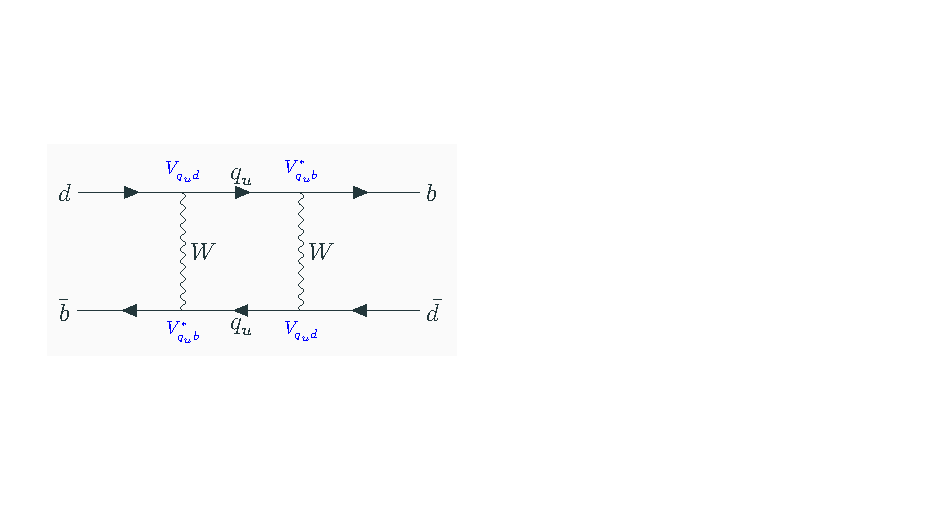
\includegraphics[width=0.6\textwidth]{content/pics/bb_oscillation.pdf}
    \caption{Transition of a $B_d^0$ meson into a $\bar{B}_d^0$ meson.}
    \label{fig:bb_oscillation}
\end{figure}

In the context of this analysis, the \textit{CP} asymmetry is calculated for the decay of $B^+$ and $B^-$ mesons. In the absence of \textit{CP} violation, 
the production rates of these two mesons are expected to be identical. Hence, a value for the \textit{CP} violation can be determined by
\begin{equation}
    A_{\mathrm{CP}} = \frac{N^+-N^-}{N^-+N^+}.
    \label{eq:CP_asymmetry}
\end{equation}
The number of observed $B^+ \rightarrow h^+h^+h^-$ is denoted as $N^+$, while the matching number of $B^- \rightarrow h^+h^-h^-$ is $N^-$.
